\chapter{First Use Case: Semantic Review Recommender}
\graphicspath{{Chapter08/Figures/}}
\label{chap:semrevrec}

During the last decade, the Web has evolved from an information space to share textual documents into a medium to distribute structured data. Linked Data\footnote{\url{http://linkeddata.org}} is a set of best practices for publishing and interlinking data on the Web and it is the base of the Web of Data, an interconnected global knowledge graph. Because of the increased amount of machine-readable knowledge freely available on the Web, there is a high interest in investigating how such information can be used to improve recommender systems~\cite{Figueroa2015}, as reviewed in Section~\ref{soa:sec:linked-data}.

Currently, most recommender systems exploit ratings to infer user preferences, although the growing popularity of social and e-commerce websites has encouraged users to write reviews. These reviews enable recommender systems to represent the multi-faceted nature of users' opinions and build a fine-grained preference model, which cannot be obtained from overall ratings~\cite{Chen2015}. Additionally, as discussed in Section~\ref{soa:sec:review-rs}, recommender systems may take advantage of reviews because they are harder to fake than ratings, are richer of information, and users may struggle to express their preference as ratings. Some studies have also documented the positive influence of product reviews on the decision processes of new users~\cite{Chatterjee2001, Kim2007}.

In this chapter, we address the issue of mining reviews and show how the extracted information, combined with Linked Data, can be exploited in recommendation tasks. On one side Linked Data can provide a rich content-based representation of the items to be recommended since they include interesting features. For example, movies represented in DBpedia\footnote{\url{http://dbpedia.org}} contain basic information such as cast and director, but also some unexpected relations, such as the fact that both \emph{Braveheart} and \emph{Saving Private Ryan} won the Best Sound Editing Academy Award. On the other side, reviews may reveal additional connections among items.
For instance, various reviews of \emph{Interstellar} mention Stanley Kubrick, although in DBpedia there is not a direct link between these two resources.
 
Therefore, we propose a new recommendation approach that semantically annotates reviews to extract useful information from them. The annotated entities and the knowledge freely available in the Web of Data are then combined to discover additional resources and generate recommendations. Our method can exploit any dataset available in the Web of Data to provide recommendations, although we rely on DBpedia and Wikidata\footnote{\url{https://www.wikidata.org}} in our implementation. 

We conducted an offline study to find the best configuration of our technique for these two datasets and comparatively evaluate our approach against a Linked Data-based and some more traditional algorithms based on ratings. We performed our study in the movie, book, and music domains, and the evaluation took into account different properties of recommender systems, that is prediction accuracy (both in terms of ratings and ranking), diversity, and novelty using a multicriteria approach. In fact, as discussed in Section~\ref{soa:sec:beyond}, not only accuracy is important: recommendations that are too obvious or already known to users may not satisfy them, although they match their taste. The results showed that our method achieved the highest diversity, provided a better accuracy than the approach based on Linked Data, and increased the novelty of recommendations with respect to collaborative filtering techniques.

More formally, the main aim of this chapter is to provide an answer to the following research questions.

\begin{description}
\item[RQ1] To what extent user reviews contain useful and non-trivial information about the items to recommend?
\item[RQ2] How such information could be enriched by exploiting a Linked Data knowledge graph for generating a list of suggested items?
\item[RQ3] Is this content-based approach more effective in terms of novelty and diversity with respect to collaborative filtering algorithms?
\end{description}

The remainder of this chapter is organized as follows. In Section~\ref{srr:sec:approach} we present our approach, while, in Section~\ref{srr:sec:eval}, we describe the evaluation method. Then, in Section~\ref{srr:sec:res}, we show the obtained results and in Section~\ref{srr:sec:discussion} we discuss them. Finally, in Section~\ref{srr:sec:concl}, we provide the conclusions.

\section{Approach}
\label{srr:sec:approach}

The architecture of SemRevRec is depicted in Figure~\ref{srr:fig:arch}. The system consists of two main modules that are highlighted with different colors: semantic annotation and discovery, and recommendation. The former is responsible for feeding the recommender system with semantically annotated entities and Linked Data through the knowledge base, while the latter provides recommendations to users. Every time a new review is submitted, the system executes the semantic annotation and discovery steps and possibly adds new entities, while the recommendation process can start when the user provides an initial item. The recommendation module works online, while the semantic annotation and discovery are done offline. Initially, some reviews are annotated and the resulting entities are used to discover additional entities through Linked Data. Each of these two modules is made up of the illustrated submodules, which are responsible for specific steps of the whole process: annotation, discovery, generation of recommendations, and their ranking. The storage of entities is not a step, but the corresponding database is a transversal submodule used by all the others. 

SemRevRec deals with the annotated or discovered entities and the items to recommend. We consider the items as a particular type of entities since SemRevRec suggests items that may be annotated or discovered entities. An item may not appear as an entity in the system, for instance a movie that was reviewed but never annotated or discovered. However, this does not mean that an entity corresponding to such a movie does not exist in the considered knowledge base. Semantic annotation and discovery steps are explained in Section~\ref{srr:sec:annotation}, while the recommendation process is presented in Section~\ref{srr:sec:recommendation}.

Although our approach is not bound to a particular domain or knowledge base available in the Web of Data, in our implementation we focus on movies, books, and music, while we rely on DBpedia and Wikidata to identify possible differences between these two knowledge bases. We chose them for annotation and discovery because they are two of the main datasets in the Web of Data and they have a vast amount of resources that belongs to a variety of domains. We used reviews from IMDb\footnote{\url{http://www.imdb.com}} for movies, LibraryThing\footnote{\url{https://www.librarything.com}} for books, and Amazon\footnote{\url{https://www.amazon.com}} for music.

\begin{figure}
\centering
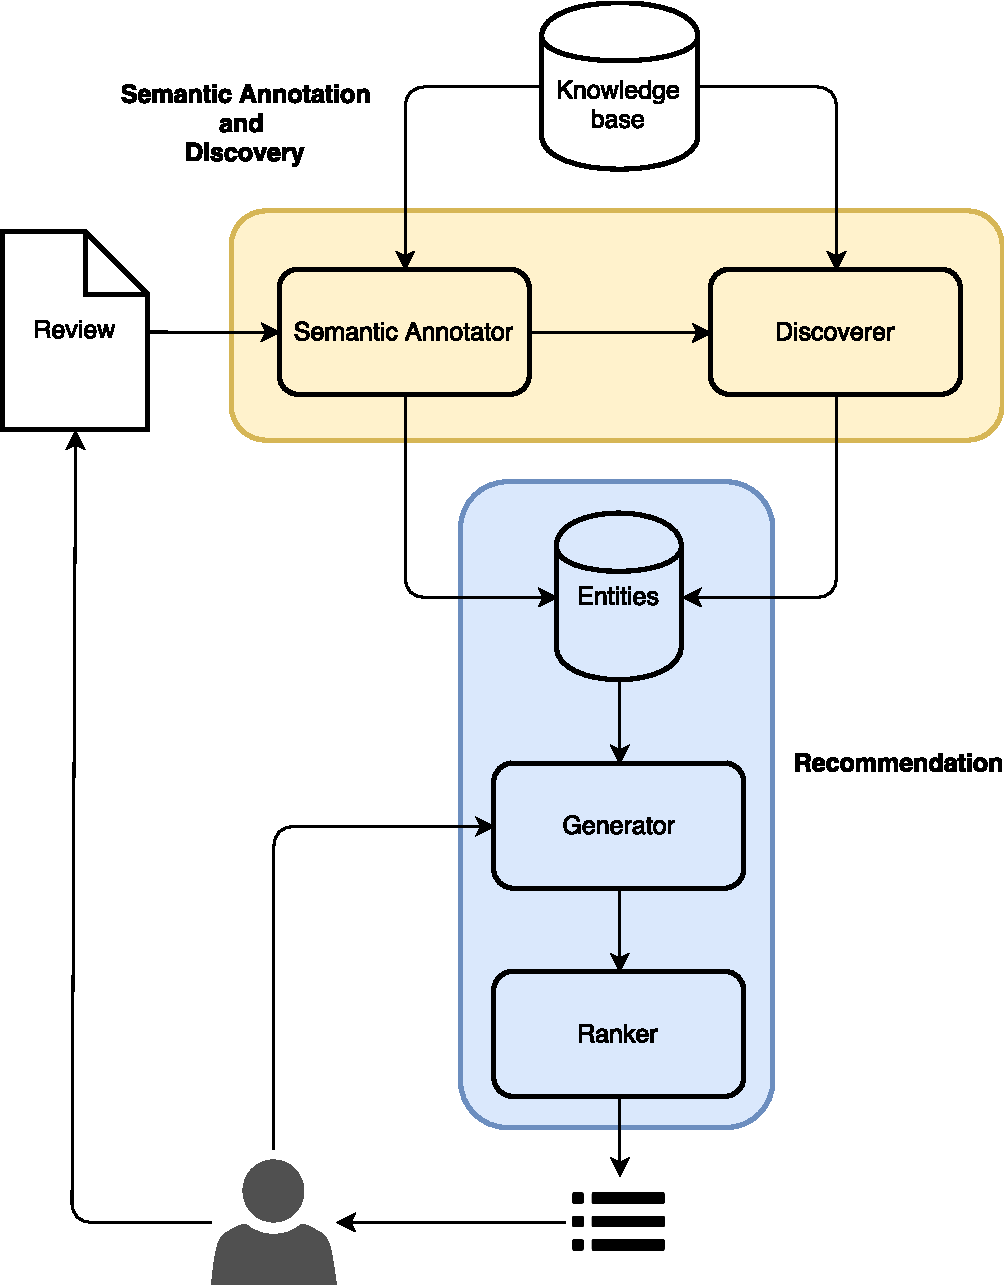
\includegraphics[width=0.65\textwidth]{architecture}
\caption[SemRevRec architecture]{The system architecture of SemRevRec.}
\label{srr:fig:arch}
\end{figure}

\subsection{Semantic Annotation and Discovery}
\label{srr:sec:annotation}

Semantic annotation is the process of annotating textual or multimedia contents with semantic tags to add information about their meaning~\cite{Saathoff2010}. In written text, this can be done by associating a URI to the recognized entities. We considered two popular semantic annotators that rely on Wikipedia: AIDA~\cite{Hoffart2011} and DBpedia Spotlight~\cite{Daiber2013}. They are both capable of disambiguating entities according to the surrounding context: this is useful because users frequently write acronyms and abbreviations. We finally selected AIDA because it is more accurate according to an independent comparison~\cite{Gangemi2013}.

The module of semantic annotation and discovery analyzes the text of the reviews and stores the identified entities in a relational database. The URI of each annotated entity is associated with the URI of the reviewed item and with the occurrence of that entity in all the reviews of that item. In fact, the same entity may appear again in reviews regarding another item. AIDA is capable of identifying and disambiguating entities mentioned in the review considering, by default, the ones available in YAGO.\footnote{\url{http://www.yago-knowledge.org}}

The YAGO resources are mapped with the equivalent ones available in DBpedia exploiting the similar structure of the URIs. For example, \texttt{yago-res:The\_Matrix} corresponds to \texttt{dbr:The\_Matrix} because their URIs where both generated starting from the title of the same Wikipedia article. In contrast, the mapping between DBpedia and Wikidata relies on the \texttt{owl:sameAs} predicate available in DBpedia. If the same entity corresponds to more than one in the other knowledge base, it is ignored in order to avoid probable inconsistencies. The same holds if there is no \texttt{owl:sameAs} property. In principle, it is also possible to perform the semantic annotation phase relying on a custom knowledge base, but AIDA is provided with a precomputed database that includes all the necessary information for annotating using YAGO. In our case, since DBpedia and Wikidata are both well interlinked with YAGO, it was less time consuming computing the mapping rather than the information needed by the annotator.

Finally, the types of each entity are obtained from the target knowledge base, optionally considering only a subset of them (for example, only the DBpedia ontology types, such as \texttt{dbo:Film}). This is done in order to minimize the amount of information retrieved and to reduce the time required for this operation. The types are stored locally because they are not expected to change often and reading them from a database is more efficient than querying the original knowledge base.

Semantic annotation allows SemRevRec to exploit Linked Data for retrieving additional entities. This is possible because the annotated entities are also resources in the Web of Data. Thus, the discoverer can find resources that are related to the annotated entities in order to enable our system to recommend more items. Reviews are a source of non-trivial relations: for example, in a movie recommendation scenario, a user can mention a movie that reminds her the reviewed one because of the colors, the setting, or the atmosphere, and these features are hardly available as Linked Data. At the same time, Linked Data can enrich information coming from users. For instance, they enable the discoverer to obtain other movies in which an actor mentioned in a review played. The discovery can take into account various properties, from more traditional ones, such as the genre, the director, or the actors, to more unexpected ones, such as other movies shot in the same place.

Given the annotated entities, the discoverer retrieves from the knowledge base other relevant entities through SPARQL queries. It relies on some properties that can be configured and depend on the domain and on the dataset considered. The discovery is not bound to a particular knowledge base or domain. On the contrary, this approach is fairly general since it relies only on RDF and SPARQL. In our implementation, we considered DBpedia and Wikidata, and we focused on movie, book, and music recommendations. Table~\ref{srr:tab:disc} summarizes the properties that we selected for discovering further items to recommend starting from the entities available in the reviews.

\begin{table}
\centering
\begin{tabular}{@{}lll@{}}
\toprule
Domain & DBpedia               & Wikidata          \\ \midrule
Movie  & \texttt{dbo:starring} & \texttt{wdt:P161} \\
Movie  & \texttt{dbo:director} & \texttt{wdt:P57}  \\
Book   & \texttt{dbo:author}   & \texttt{wdt:P50}  \\
Music  & \texttt{dbo:artist}   & \texttt{wdt:P175} \\
Music  & \texttt{dbo:writer}   & \texttt{wdt:P676} \\ \bottomrule
\end{tabular}
\caption[Properties for discovery phase]{The properties considered for the discovery phase.}
\label{srr:tab:disc}
\end{table}

More specifically, the discoverer reads the annotated entities stored during the semantic annotation phase. The discoverer is able to obtain all the resources that have the given entities as an object of the selected properties. For example, in the movie domain, we selected \texttt{dbo:starring} and \texttt{dbo:director} in the case of DBpedia because most of the annotated properties, when not movies, were actors and directors. This allows the system to discover other movies from the same director or actor named in a given review. Sometimes directors or actors not involved in the movie were also mentioned for comparison. The discoverer can retrieve other movies from these entities that are relevant for the user who wrote the review, thus can also be of interest for other users. Similarly to movies, we selected \texttt{dbo:author} for books as well as \texttt{dbo:artist} and \texttt{dbo:writer} for music because most of the annotated entities were authors, artists or writers when not books and songs, respectively. It is possible to exploit both direct and inverse properties.
 
The discoverer stores the discovered entities in a relational database for efficiency reasons. The URI of each discovered entity is associated with the URI of the annotated entity through which it was discovered, and, optionally, with the LDSD measure~\cite{Passant2010} between them. This measure is inversely proportional to the number of links between two resources: more links result in a lower distance. Each discovered entity may be found through more than a single annotated entity. The LDSD can be exploited in the ranking phase, which is described in Section~\ref{srr:sec:ranking}. However, since its computation is expensive due to the various SPARQL queries involved, it may be optionally skipped to speed up the discovery step. Obviously, in this case, the LDSD measure does not contribute to the ranking.

\subsection{Recommendation}
\label{srr:sec:recommendation}

The recommendation process consists of two main steps: the generation of the candidate recommendations and their ranking. Given an initial item, SemRevRec retrieves all the entities that are related to the initial item and then ranks them.

Firstly, the system selects the annotated entities that were mentioned in the reviews of the initial item. Afterwards, it obtains the entities that mention the initial item, that is entities whose reviews generated an annotated entity that corresponds to the initial item. For example, if the initial item is \emph{Interstellar} and a review of \emph{2001: A Space Odyssey} mention \emph{Interstellar}, then \emph{2001: A Space Odyssey} is considered as a candidate recommendation.

Secondly, SemRevRec optionally retrieves the discovered entities. They may include entities discovered through the initial item. For instance, if the initial item is \emph{Interstellar} and \emph{The Dark Knight} was previously discovered because both these movies have been directed by Christopher Nolan, \emph{The Dark Knight} is selected. The same holds if \emph{Interstellar} was discovered from \emph{The Dark Knight}, that is Christopher Nolan was annotated in the reviews of the latter. Similarly, the entities discovered through other entities that were annotated in the reviews of the initial item are relevant. For example, if \emph{Interstellar} is the initial item, Stanley Kubrick was annotated in one of its reviews, and \emph{2001: A Space Odyssey} was discovered through Stanley Kubrick, then \emph{2001: A Space Odyssey} is a candidate recommendation.

It is possible to configure the generator to include in the candidate recommendations the discovered entities or not. It is also possible to specify the minimum occurrence required for entities to be included in the candidate recommendation set, which is expressed as a percentage of the maximum occurrence of entities in the reviews of the item considered.

\subsection{Ranking Functions}
\label{srr:sec:ranking}

Finally, SemRevRec ranks the candidate recommendations. We defined three different ranking functions. The first one is presented in Equation~\ref{srr:eq:r1} and takes into account only the occurrence $occur(i)$ of the entities available in the reviews. $occur(i)$ is equal to the number of reviews of an initial item $i_{in}$ where an entity $i$ is annotated plus the number of reviews of $i$ where $i_{in}$ is annotated (if any). However, the entity $i$ can be annotated or discovered. For the latter, the occurrence of the entity through which it was discovered is used. The $\alpha$ coefficient is $1$ if $i$ is an annotated entity. Otherwise, it can be configured to a custom value (the default is $0.5$) to weight the contribution of a discovered entity to the ranking. To obtain a value between $0$ and $1$, R1 is normalized to the maximum occurrence of entities $j$ that belong to the candidate recommendation set $CR$.

\begin{equation}
\label{srr:eq:r1}
\mathit{R1}(i) = \frac{\alpha \cdot \mathit{occur(i, i_{in})}}{max_{j \in \mathit{CR}}(\mathit{occur(j, i_{in})})}
\end{equation}

The second ranking function (Equation~\ref{srr:eq:r2}) also considers the LDSD measure between each discovered entity and the entity through which it was discovered. This avoids assigning the same value to all the entities discovered through the same annotated entity as R1 does. 
As for R1, the entity $i$ can be annotated or discovered. The $\beta$ coefficient is $1$ if $i$ is an annotated entity, $0.5$ otherwise. The $\gamma$ coefficient is $0.5$ for discovered entities, $0$ otherwise. In this way, R2 returns a number between $0$ and $1$, which is equal to R1 for the annotated entities, while, for the discovered entities, it is the average of R1 and $LDSD(i,i_o)$, where $i_o$ is the entity through which $i$ was discovered.

\begin{equation}
\label{srr:eq:r2}
\mathit{R2}(i) = \beta \cdot \mathit{R1}(i) + \gamma \cdot (1 - \mathit{LDSD}(i, i_o))
\end{equation}

The third ranking function (Equation~\ref{srr:eq:r3}) considers the LDSD measure between an entity $i$ and the initial item $i_{in}$. The coefficients $\eta$ and $\kappa$ can be set to custom values and they allow the ranker to weight differently the contribution of the occurrence in the review (given by R2) and Linked Data (through the LDSD).

\begin{equation}
\label{srr:eq:r3}
\mathit{R3}(i) = \eta \cdot \mathit{R2}(i) + \kappa \cdot (1- \mathit{LDSD}(i, i_{in}))
\end{equation}

LDSD measures between discovered entities and the entities through which they were discovered need to be precomputed at discovery time (see Section~\ref{srr:sec:annotation}) to enable SemRevRec to exploit R2, LDSD measures between entities in $CR$ and the initial item need to be computed while ranking.% In the latter case, the ranking time is increased.

\section{Evaluation Procedure}
\label{srr:sec:eval}

We evaluated the performance of SemRevRec with two offline experiments conducted in the movie, book, and music domains. The purpose of the first experiment is to understand the impact of the ranking function, the discovery, the occurrence threshold, and the coefficients of R3. Furthermore, we performed the first experiment two times, first relying on DBpedia and then on Wikidata, to assess the effect of the knowledge base on the quality of the recommended items. The aim of the second experiment is to compare our proposal with traditional recommendation techniques that rely on ratings and a recommender system based on Linked Data.

For conducting both experiments, we obtained from IMDb, LibraryThing, and Amazon the user reviews regarding all the items included in the MovieLens~1M,\footnote{\url{http://grouplens.org/datasets/movielens/1m/}} the LibraryThing\footnote{\url{http://www.macle.nl/tud/LT/}} and the HetRec 2011 LastFM\footnote{\url{http://ir.ii.uam.es/hetrec2011/datasets/lastfm/readme.txt}} datasets of user ratings.

The items of such rating datasets were mapped with the corresponding entities available in DBpedia relying on the work of Di Noia et al.~\cite{DiNoia2016}. Furthermore, their equivalent entities in Wikidata were obtained from DBpedia itself, as described in Section~\ref{srr:sec:annotation}. For the purpose of retrieving the user reviews, Wikidata was exploited in order to discover the IMDb identifiers of the movies available in the MovieLens~1M dataset. On the contrary, the LibraryThing dataset already contained the references useful for obtaining the reviews. Regarding the musical artists present in the HetRec 2011 LastFM dataset, we relied on the search feature of Amazon for identifying their most reviewed musical work.

\begin{table}
\centering
\begin{tabular}{@{}lrrr@{}}
\toprule
                   & Movie     & Book         & Music   \\ \midrule
Users              & 6,040     & 7,279        & 1,892   \\
Items              & 3,706     & 37,232       & 17,632  \\
Ratings            & 1,000,209 & 2,056,487    & 92,834  \\
Reviews            & 559,858   & 363,791      & 669,978 \\
Distinct entities  & 107,468   & 77,120       & 70,762  \\
Total entities     & 574,435   & 303,705      & 296,777 \\ \bottomrule
\end{tabular}
\caption[Statistics about datasets and reviews]{Statistics about the available datasets and reviews.}
\label{srr:tab:stats}
\end{table}

\begin{figure}
\centering
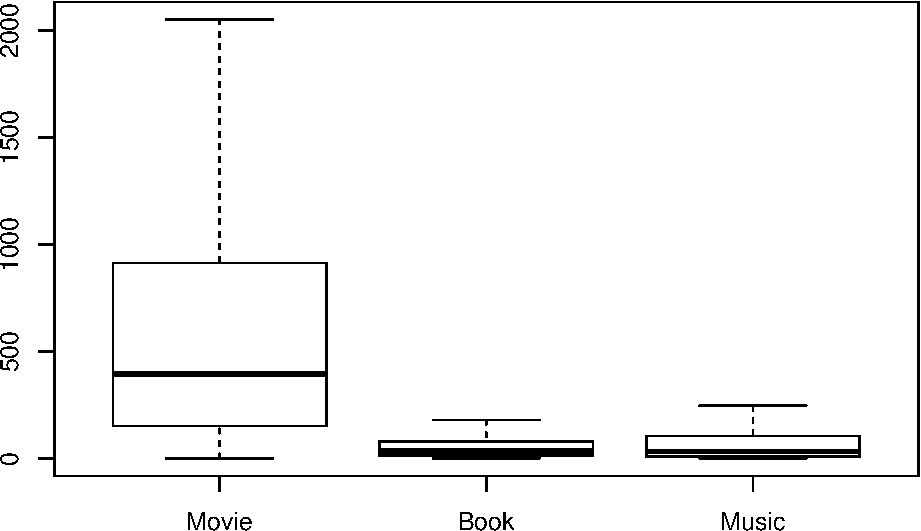
\includegraphics[width=0.85\textwidth]{boxplot}
\caption[Entities extracted from the reviews]{Distribution of entities extracted from the reviews per domain.}
\label{srr:fig:boxplot}
\end{figure}

Table~\ref{srr:tab:stats} lists several statistics regarding the exploited rating datasets and the analyzed reviews in the three domains considered. It is worth noting that the LastFM dataset contains a limited number of ratings with respect to the other datasets and, for this reason, it is the most sparse one. The LibraryThing dataset includes a considerable number of items, even if fewer reviews are available in the book domain. Regarding the outcome of the semantic annotation, the number of distinct and total entities identified in user reviews is reported. The ratio between these two values may be considered a measure of the variety of the mentioned topics. According to this measure, the reviews about movies are the most varied ones in terms of entities.

Figure~\ref{srr:fig:boxplot} displays the boxplots representing the distributions of the number of annotated entities per each item according to the domain, excluding the outliers for graphical reasons. Given the interquartile range $IQR = Q3 - Q1$, all data points not belonging to the interval $(Q1 - 1.5 \cdot IQR; Q3 + 1.5 \cdot IQR)$ are considered outliers. It is clear that movie reviews are fairly different from the other ones. This may be related to the higher ratio between reviews and items in the movie domain.

We relied on a 5-fold cross-validation in order to perform the evaluations. We considered ratings positive if their score was greater than~3 on a scale from 1 to~5 for MovieLens, greater than 6 on a scale from 1 to~10 for LibraryThing, and greater than~0 for LastFM. In fact, the latter dataset contains implicit feedback, while the others are examples of explicit feedback. Exploiting the lists of the top-10 recommendations for each user, we computed the measures of precision, recall, nDCG, Entropy Based Novelty (EBN)~\cite{Bellogin2010}, and diversity~\cite{Zhang2008}.

For the implementation, we rely on the LibRec library.\footnote{\url{https://www.librec.net}} It computes measures according to the \emph{all unrated items} protocol \cite{Steck2013}. More specifically, it creates a top-$k$ recommendation list for each user by predicting a score for every item not rated by that particular user, whether that item appears in the user test set or not. All the non-rated items are considered to be irrelevant for the user. This explains the low values for the measures (in particular precision and recall) as the quality of recommendations tend to be underestimated. However, Steck \cite{Steck2013} suggests to rely on this protocol rather than the \emph{rated test-items}, which includes only rated test items in the top-$k$ list, as the user satisfaction regarding top-$k$ recommendations depends on the ranking of all items.

\section{Evaluation Results}
\label{srr:sec:res}

We report the results of the first experiment on optimizing the parameters of our SemRevRec system in Section~\ref{srr:sec:exp1}. The results of comparing our approach with baselines from related work are documented in Section~\ref{srr:sec:exp2}.

\subsection{Optimizing the SemRevRec Parameters}
\label{srr:sec:exp1}

In this experiment, we evaluated the impact of the ranking function, the discovery, the occurrence threshold, and the coefficients of R3 on the performance of our algorithm. We executed SemRevRec in three domains with different ranking functions with and without the discovery phase. We also varied the configuration parameters $\eta$ and $\kappa$ of the ranking function R3, in order to identify possible relationships between the occurrence and the LDSD measure. Furthermore, we considered how the percentage of the minimum occurrence required for entities to be included in the candidate recommendation set impacts on the results. The main configurations tested are listed in Table~\ref{srr:tab:config}.

\begin{table}
\centering
\begin{tabular}{@{}llllll@{}}
\toprule
Conf. & Ranking & Discovered & Occurrence & $\eta$ & $\kappa$ \\ \midrule
C1    & R1      & False      & 0.05       & --     & --       \\
C2    & R1      & True       & 0.05       & --     & --       \\
C3    & R2      & False      & 0.05       & --     & --       \\
C4    & R2      & True       & 0.05       & --     & --       \\
C5    & R3      & False      & 0.05       & 0.50   & 0.50     \\
C6    & R3      & True       & 0.05       & 0.50   & 0.50     \\
C7    & R3      & True       & 0.05       & 0.75   & 0.25     \\
C8    & R3      & True       & 0.05       & 0.25   & 0.75     \\
\bottomrule 
\end{tabular}
\caption[Configuration parameters of SemRevRec]{The configuration parameters of SemRevRec.}
\label{srr:tab:config}
\end{table}

Table~\ref{srr:tab:ex1-ml}, Table~\ref{srr:tab:ex1-lt}, and Table~\ref{srr:tab:ex1-fm} summarize the results obtained with the DBpedia knowledge base in the movie, book, and music domain. For all the measures but EBN, higher values represent better results, while the lower is EBN, the higher is the novelty. The best values and configurations are highlighted in boldface.\footnote{More values are highlighted for the same measure if the differences among them are not statistically significant.} For deciding if the difference between two measures was statistically significant, we relied on the Welch's \emph{t}-test (or unequal variances \emph{t}-test), an adaptation of the Student's \emph{t}-test more reliable when the two samples have unequal variances and unequal sample sizes~\cite{Ruxton2006}. We considered \emph{p}~<~0.001 because we applied the Bonferroni correction as we performed pairwise comparisons.

The obtained results suggest that the discovery of additional entities through Linked Data is useful for improving the precision of the recommended items. In fact, the best configurations in all the domains but music (C8 for movies, C2 for books) rely on it. In the music domain there is not a significant difference in the measures when relying on the discovery phase. This may be related to the fact that we considered reviews about musical works in order to recommend musical artists.

The best ranking function depends instead on the domain. For movies, R3 outperformed the other rankers (C8), while, for book and music recommendations, R1 accounts for the best results (C2), although in the music domain the values obtained with R1 and R2 were equivalent (C4). This suggests that a simpler ranker may be more effective on sparse data, and it could be better to rely on information from reviews than on Linked Data. Additionally, the coefficients $\eta$ and $\kappa$ of R3 may have a high impact on the results as shown by C6, C7, and C8 in Table~\ref{srr:tab:ex1-ml}, even if, in the music domain, the measures do not vary. In particular, C8 improves significantly the precision and recall measures with respect to other configurations of R3 in the movie and book domains.

\begin{table}
\centering
\begin{tabular}{@{}lrrrrr@{}}
\toprule
Conf.       & Precis.         & Recall          & nDCG            & EBN             & Divers. \\ \midrule
C1          & 0.0604          & 0.0399          & 0.0412          & 1.2804          & \textbf{0.2431} \\
C2          & 0.0529          & 0.0327          & 0.0343          & 1.2776          & 0.1629  \\
C3          & 0.0604          & 0.0399          & 0.0412          & 1.2804          & \textbf{0.2431} \\
C4          & 0.0276          & 0.0178          & 0.0197          & \textbf{0.7820} & 0.1716  \\
C5          & \textbf{0.0683} & 0.0424          & 0.0491          & 1.0047          & 0.1795  \\
C6          & 0.0460          & 0.0255          & 0.0320          & 0.9354          & 0.1794  \\
C7          & 0.0344          & 0.0191          & 0.0243          & 0.8248          & 0.1464  \\
\textbf{C8} & \textbf{0.0711} & \textbf{0.0478} & \textbf{0.0524} & 1.0163          & 0.2114  \\ \bottomrule
\end{tabular}
\caption[Experimental results with MovieLens and DBpedia]{Experimental results obtained with MovieLens and DBpedia.}
\label{srr:tab:ex1-ml}
\end{table}

\begin{table}
\centering
\begin{tabular}{@{}lrrrrr@{}}
\toprule
Conf.       & Precis.         & Recall          & nDCG            & EBN             & Divers. \\ \midrule
C1          & 0.0396          & 0.0350          & 0.0341          & 0.4081          & 0.7701  \\
\textbf{C2} & \textbf{0.0506} & \textbf{0.0497} & \textbf{0.0465} & 0.2771          & 0.7780  \\
C3          & 0.0396          & 0.0350          & 0.0341          & 0.4081          & 0.7701  \\
C4          & 0.0357          & 0.0340          & 0.0353          & \textbf{0.1946} & 0.8919  \\
C5          & 0.0462          & 0.0373          & \textbf{0.0462} & 0.2809          & 0.8663  \\
C6          & 0.0356          & 0.0331          & 0.0366          & 0.2280          & 0.9039  \\
C7          & 0.0306          & 0.0269          & 0.0317          & 0.2444          & 0.8932  \\
C8          & 0.0421          & 0.0418          & \textbf{0.0429} & 0.2077          & \textbf{0.9118} \\ \bottomrule
\end{tabular}
\caption[Experimental results with LibraryThing and DBpedia]{Experimental results obtained with LibraryThing and DBpedia.}
\label{srr:tab:ex1-lt}
\end{table}

\begin{table}
\centering
\begin{tabular}{@{}lrrrrr@{}}
\toprule
Conf.       & Precis.         & Recall          & nDCG            & EBN             & Divers. \\ \midrule
\textbf{C1} & \textbf{0.0495} & \textbf{0.0504} & \textbf{0.0486} & 0.7894          & 0.5654  \\
\textbf{C2} & \textbf{0.0504} & \textbf{0.0515} & \textbf{0.0473} & 0.6640          & 0.6021  \\
\textbf{C3} & \textbf{0.0495} & \textbf{0.0504} & \textbf{0.0486} & 0.7894          & 0.5654  \\
\textbf{C4} & \textbf{0.0504} & \textbf{0.0515} & \textbf{0.0473} & 0.6640          & 0.6022  \\
C5          & 0.0363          & 0.0371          & 0.0378          & 0.2619          & 0.9238  \\
C6          & 0.0360          & 0.0370          & 0.0378          & \textbf{0.2422} & \textbf{0.9325}  \\
C7          & 0.0361          & 0.0369          & 0.0378          & \textbf{0.2425} & \textbf{0.9325}  \\
C8          & 0.0360          & 0.0368          & 0.0378          & \textbf{0.2411} & \textbf{0.9329} \\ \bottomrule
\end{tabular}
\caption[Experimental results with LastFM and DBpedia]{Experimental results obtained with LastFM and DBpedia.}
\label{srr:tab:ex1-fm}
\end{table}

\begin{figure}
\centering
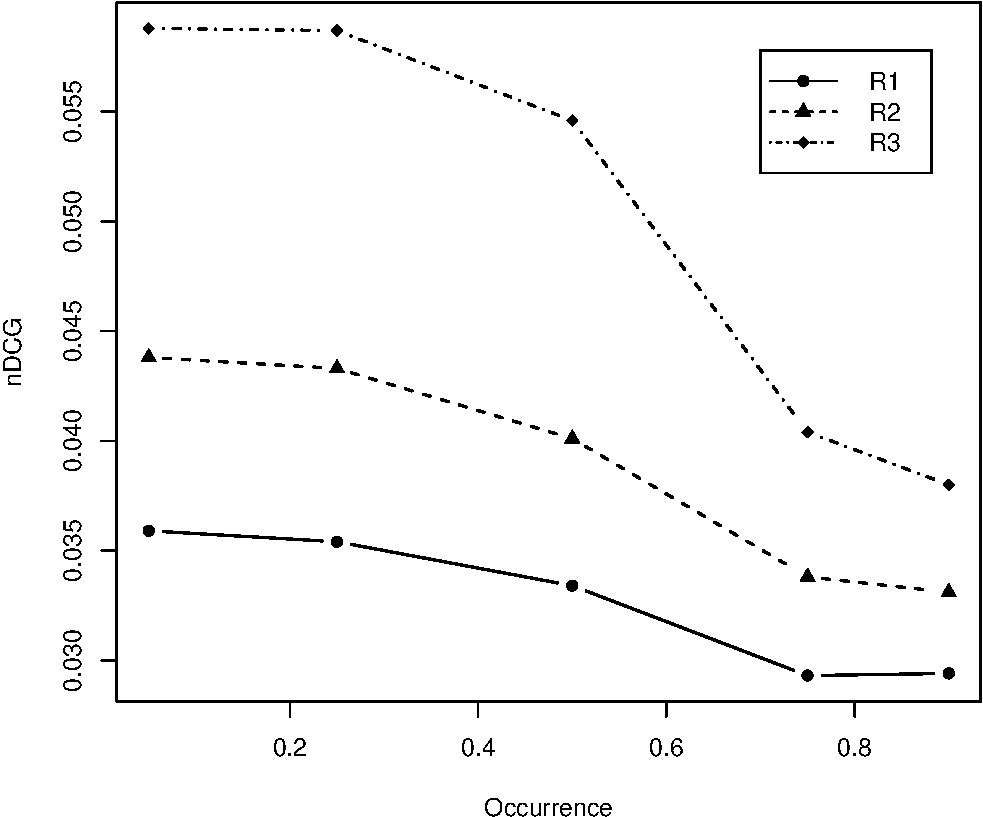
\includegraphics[width=0.75\textwidth]{lineplot}
\caption[nDCG with MovieLens and Wikidata]{The nDCG score obtained by varying the number of entities considered with MovieLens and Wikidata.}
\label{srr:fig:lineplot}
\end{figure}

Figure~\ref{srr:fig:lineplot} illustrates the performance in terms of nDCG of the three ranking functions available in SemRevRec when the number of entities considered for the recommendation process varies. The occurrence represents the minimum number of times an entity needs to be annotated in the reviews of a certain item in order to be included in the candidate recommendation set. It is expressed as a percentage of the most annotated entity for an item. The plot is based on the results obtained in the movie domain with the Wikidata knowledge base, as this can be considered the most representative case. Unsurprisingly, all rankers tend to converge, as the number of entities available decreases. However, it is important to notice that the nDCG is monotonically decreasing. This fact happens in the majority of the domains with both knowledge bases and supports the hypothesis that the higher is the number of available entities, the better is the quality of the recommendations.

\begin{sidewaysfigure}[p]
\centering
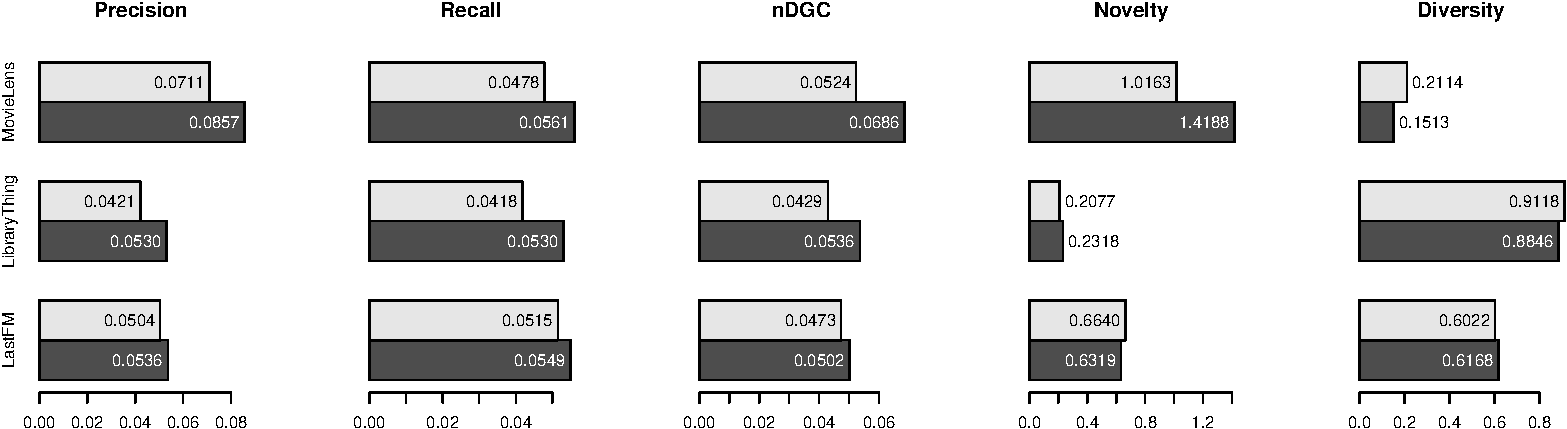
\includegraphics[width=\textwidth]{barplot}
\caption[Comparison between DBpedia and Wikidata]{A comparison between DBpedia and Wikidata. Light grey represents DBpedia, dark grey Wikidata.}
\label{srr:fig:barplot}
\end{sidewaysfigure}

Figure~\ref{srr:fig:barplot} compares the results obtained by the best configuration of our algorithm when using DBpedia and Wikidata for each domain. Although both knowledge bases are derived from Wikipedia, the results differ. In particular, Wikidata outperformed DBpedia in the vast majority of the considered measures. A possible reason may be that Wikidata provides higher data quality for the recommendation task, as it also contains knowledge manually encoded by human editors. At the instance level, this may be primary due to the interlinking of resources since we rely on the LDSD measure that exploits direct and indirect links. At the ontology level, the properties considered in the discovery may also have an high impact. We should investigate which features of a knowledge base are well suited for a Linked Data-based recommender system, although they can also depend on the particular domain considered.

Table~\ref{srr:tab:ex1-wd} lists the results obtained with Wikidata. They vary significantly when the $\eta$ and $\kappa$ weights of the ranking function R3 are changed. Thus, we decided to include in this chapter only the results related to the configurations C4, C6, C7, and C8, although we tested all the ones listed in Table~\ref{srr:tab:config}. The complete evaluation is available on the Web.\footnote{\url{https://doi.org/10.6084/m9.figshare.5074081}} In general, Wikidata provides better results with respect to DBpedia and this behavior is consistent in all domains, but differences are more significant when movies are recommended.

\begin{table}
\centering
\begin{tabular}{@{}llrrrrr@{}}
\toprule
Conf. & Domain  & Precis. & Recall & nDCG   & EBN    & Divers. \\ \midrule
C4    & Movie   & 0.0582  & 0.0368 & 0.0438 & \textbf{1.3626} & 0.1223 \\
C6    & Movie   & 0.0757  & 0.0487 & 0.0588 & 1.4284 & \textbf{0.1461} \\
C7    & Movie   & 0.0728  & 0.0459 & 0.0552 & 1.4322 & \textbf{0.1423} \\
\textbf{C8} & \textbf{Movie} & \textbf{0.0857} & \textbf{0.0561} & \textbf{0.0686} & 1.4188 & \textbf{0.1513} \\
\midrule
C4    & Book   & 0.0392   & 0.0373 & 0.0379 & 0.2634 & 0.8455  \\
C6    & Book   & 0.0452   & 0.0443 & 0.0466 & 0.2621 & 0.8705  \\
C7    & Book   & 0.0365   & 0.0334 & 0.0380 & 0.2809 & 0.8600  \\
\textbf{C8} & \textbf{Book}  & \textbf{0.0530} & \textbf{0.0530} & \textbf{0.0536} & \textbf{0.2318} & \textbf{0.8846} \\
\midrule
\textbf{C4} & \textbf{Music} & \textbf{0.0536} & \textbf{0.0549} & \textbf{0.0502} & 0.6319 & 0.6168 \\
C6    & Music  & 0.0384   & 0.0395 & 0.0375 & \textbf{0.3083} & \textbf{0.9314} \\
C7    & Music  & 0.0390   & 0.0401 & 0.0380 & \textbf{0.3062} & \textbf{0.9327} \\
C8    & Music  & 0.0367   & 0.0377 & 0.0363 & \textbf{0.3178} & \textbf{0.9322} \\ \bottomrule
\end{tabular}
\caption[Experimental results with Wikidata]{Experimental results obtained with Wikidata.}
\label{srr:tab:ex1-wd}
\end{table}

\subsection{Comparison with Baselines}
\label{srr:sec:exp2}

We compared our technique to the Most Popular, Random Guess, Item KNN, and Bayesian Personalized Ranking (BPR)~\cite{Rendle2009} algorithms, as implemented in LibRec, and with SPrank~\cite{DiNoia2016}, a state-of-the-art Linked Data-based recommender. We set the neighborhood size for Item KNN to 80, while we used 100 factors for BPR, as done by Musto et al.~\cite{Musto2016}. We configured SPrank to exploit LambdaMart as the ranking method and to follow in the DBpedia graph the same properties that we selected for our algorithm, as listed in Table~\ref{srr:tab:disc}.

Table~\ref{srr:tab:ex2-ml}, Table~\ref{srr:tab:ex2-lt}, and Table~\ref{srr:tab:ex2-fm} list the results obtained in the movie, book, and music domain, respectively. The best values are highlighted in boldface.\footnote{More values are highlighted for the same measure if the differences among them are not statistically significant. In the case of EBN and diversity, when Random Guess was the best, we also highlighted the second best because its precision, recall, and nDCG were close to zero. This means that the recommendations provided are completely unrelated and their novelty and diversity are not relevant.} For SemRevRec, we reported both the configuration with the best trade-off among the various measures and the best scores achieved for each measure in the experiment described in Section~\ref{srr:sec:exp1}. In all the experimental trails, SemRevRec provided the best diversity and a better accuracy (both in rating prediction and ranking) than SPrank, while it improved in novelty with respect to traditional techniques. BPR accounted for the highest precision, recall, and nDCG. In general, the diversity is rather low for movies, while for music and books is above 0.6, apart for Item KNN.

The differences between SemRevRec and the other approaches are statistically significant according to the Welch's \emph{t}-test with \emph{p}~<~0.001, except for SPrank, BRP, Most Popular, and Random Guess in the movie domain regarding the measure of diversity, SPrank in the book domain regarding the measures of precision and diversity, and Most Popular in the music domain regarding the measure of diversity.

\begin{table}
\centering
\begin{tabular}{@{}lrrrrr@{}}
\toprule
Algorithm & Precis. & Recall & nDCG   & EBN    & Divers. \\ \midrule
SemRevRec & 0.0857  & 0.0561 & 0.0686 & 1.4188 & 0.1513 \\
-- Best Scores & 0.0857 & 0.0561 & 0.0686 & \textbf{0.7820} & \textbf{0.2431} \\ \midrule
SPrank    & 0.0445  & 0.0254 & 0.0280 & 0.8813 & 0.1612 \\
Item KNN  & 0.1626  & 0.1105 & 0.1302 & 2.6846 & 0.0696 \\
BPR       & \textbf{0.2347}  & \textbf{0.1737} & \textbf{0.1930} & 1.8358 & 0.1769 \\
Popular   & 0.1325  & 0.0840 & 0.0969 & 2.7439 & 0.1412 \\
Random    & 0.0055  & 0.0028 & 0.0031 & \textbf{0.3018} & 0.1679 \\ \bottomrule
\end{tabular}
\caption[Comparison using the MovieLens dataset]{Experimental comparison using the MovieLens dataset.}
\label{srr:tab:ex2-ml}
\end{table}

\begin{table}
\centering
\begin{tabular}{@{}lrrrrr@{}}
\toprule
Algorithm & Precis. & Recall & nDCG   & EBN    & Divers. \\ \midrule
SemRevRec & 0.0530  & 0.0530 & 0.0536 & 0.2318 & 0.8846 \\
-- Best Scores & 0.0530  & 0.0530 & 0.0536 & 0.1946 & \textbf{0.9118} \\ \midrule
SPrank    & 0.0379  & 0.0346 & 0.0337 & \textbf{0.1562} & 0.8037 \\
Item KNN  & 0.0620  & 0.0564 & 0.0662 & 1.4956 & 0.2259 \\
BPR       & \textbf{0.0862}  & \textbf{0.0817} & \textbf{0.0895} & 0.6043 & 0.7177 \\
Popular   & 0.0423  & 0.0343 & 0.0447 & 1.6034 & 0.6483 \\
Random    & 0.0004  & 0.0002 & 0.0003 & \textbf{0.0382} & \textbf{0.9879} \\ \bottomrule
\end{tabular}
\caption[Comparison using the LibraryThing dataset]{Experimental comparison using the LibraryThing dataset.}
\label{srr:tab:ex2-lt}
\end{table}

\begin{table}
\centering
\begin{tabular}{@{}lrrrrr@{}}
\toprule
Algorithm & Precis. & Recall & nDCG   & EBN    & Divers. \\ \midrule
SemRevRec & 0.0536  & 0.0549 & 0.0502 & 0.6319 & 0.6168 \\
-- Best Scores & 0.0536  & 0.0549 & 0.0502 & 0.2411 & \textbf{0.9329} \\ \midrule
SPrank    & 0.0156  & 0.0158 & 0.0176 & \textbf{0.1834} & 0.9077 \\
Item KNN  & 0.1392  & 0.1428 & 0.1720 & 1.6023 & 0.4730 \\
BPR       & \textbf{0.1545}  & \textbf{0.1583} & \textbf{0.1808} & 0.9404 & 0.6547 \\
Popular   & 0.0686  & 0.0703 & 0.0791 & 2.0360 & 0.6519 \\
Random    & 0.0005  & 0.0005 & 0.0004 & \textbf{0.0442} & \textbf{0.9946} \\ \bottomrule
\end{tabular}
\caption[Comparison using the LastFM dataset]{Experimental comparison using the LastFM dataset.}
\label{srr:tab:ex2-fm}
\end{table}

\section{Discussion}
\label{srr:sec:discussion}

In general, the results obtained by our algorithm in the music and book domains are not as good as the ones achieved with movie recommendations. This may be due to the characteristics of the reviews, as illustrated in Figure~\ref{srr:fig:boxplot} and previously discussed. The entities annotated for each item in these two domains are much less than the entities available in movie reviews. This fact should be further studied. Furthermore, it would be interesting to investigate the impact of the number of reviews available and their quality with respect to the recommendation process. For example, a meaningful album review mentions the author and similar albums or artists the user liked, while a review describing the package is not very useful in our scenario. In fact, we aim to suggest other artists to listen to, although packaging may impact on the decision of buying a physical copy of that album. Finally, the significant difference in the results obtained when exploiting Wikidata or DBpedia suggests that the impact of knowledge bases, notably the selection of types and properties exploited, on the performance should be further analyzed.

In this work, we relied on all the reviews available for the items present in the rating datasets used for the evaluation. However, only reviews about some items, for example the ones with the average rating higher than a threshold, or only some reviews for each item, for example only the ones that are rated positively, could be considered during the semantic annotation phase. Nevertheless, lower performance on music artists and books was expected because the available ratings were more sparse than the ones regarding movies. This holds for all the algorithms and explains the general difference of scores in these domains. 

SemRevRec showed the best diversity. In the sparse dataset of books, it achieved precision, recall, and nDCG comparable to Item KNN with a much higher diversity, although the former is a content-based method. Collaborative filtering techniques are known to suffer less of the overspecilization problem and provide better rating prediction and ranking than content-based ones. For this reason, although collaborative filtering is very popular, we decided to include in the baseline a technique among many, that is BPR, one of the newest and most promising. Nevertheless, it showed a lower diversity than our algorithm. Not surprisingly, it also accounted for the best rating prediction and ranking. 

Our approach also provided a higher novelty than traditional techniques and a better rating prediction and ranking than SPrank. In the movie domain, SemRevRec accounted for the best novelty, while with music and books for the second best, with results close to SPrank. Additionally, when optimized for this measure, SemRevRec had similar or higher rating prediction and ranking than SPrank. On the contrary, when the former is optimized for rating prediction and ranking, it could be preferred to the latter to increase the novelty of recommendations, while also limiting the loss in rating prediction and ranking.

Finally, SemRevRec was evaluated considering the recommendations generated for all the previous items a user liked, as its generation approach is rather naive and it takes into account only an initial item. Combining it with a machine learning technique could significantly improve its performance, but further experiments are required to prove this.

\section{Conclusion}
\label{srr:sec:concl}

In this chapter we proposed a novel recommendation approach based on the semantic annotation of user reviews and Linked Data. We conducted an offline study of the recommender system in the movie, book, and music domains, which showed that our method provides the best diversity. It also improved rating prediction and ranking compared to another algorithm based on Linked Data, while it increased the novelty of recommendations with respect to traditional techniques. Furthermore, we tested our approach with different knowledge bases and Wikidata systematically achieved better results than DBpedia. Although the reviews available for the book and music domains seem to contain a smaller amount of useful information, the results of the offline study suggest that our algorithm can provide more diverse recommendations and reach an interesting compromise between the accuracy and the novelty of the suggested items.

This work represents a practical application of multicriteria evaluation approaches, but it also raises further interesting research issues that still need to be properly addressed. For this reason, we intend to investigate in greater details how the nature of the user reviews influences the performance of our algorithm. Furthermore, the significant difference in the results obtained when exploiting Wikidata or DBpedia suggests that too little is known about how knowledge bases (notably their types and properties) might impact on the performance of Linked Data-based recommender systems. We also plan to take into account the sentiment of the reviews, that is whether the overall opinion on the item reviewed is positive or negative. Finally, we are evaluating applications of our approach on textual resources different than reviews, for example research papers or their abstracts. In this case sentiment would not be relevant, while annotated entities could be concepts representing the main topics addressed in the document.
